\chapter{Aircraft Fuel System}
\label{chap:fuelSystem}

\section{Case Description}

The fuel system on-board aircraft is a complex system where fuel must
be transferred between multiple tanks to ensure the engines always have
a sufficient supply of fuel and that the aircraft is in balance. An
overview of the fuel tanks and how they are connected can be seen in
Fig~\ref{fig:fuelTanks}.

\begin{figure}[!ht]
\centering
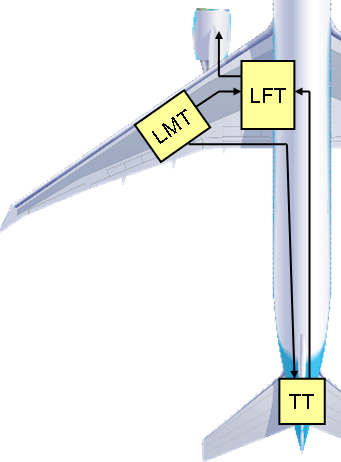
\includegraphics[width=4.5cm]{fuelSystem/FuelTanks.png}
\caption{Overview of the fuel tanks in the case
  study \label{fig:fuelTanks}}
\end{figure}

In the real system, tanks are also placed symmetrically in the
right-hand side of the aircraft --- these have been abstracted away in
the model.

At takeoff, the Trimmer Tank (TT) placed in the rear end of the
aircraft must be empty for safety reasons, but once cruise altitude
has been reached the trimmer tank must be filled to distribute weight
and therefore obtain better balance of the aircraft. The Left Feeder
Tank (LFT) must always have sufficient supply of fuel to the engine
which continuously consumes fuel (more during takeoff than at cruise
altitude). If the level of fuel in the feeder tank reaches a minimum
threshold fuel must be pumped from the Left Middle Tank (LMT) to the
feeder tank. If the middle tank becomes empty, fuel must be transferred
from the trimmer tank to ensure a sufficient level of fuel for the
engine. Finally, before landing the aircraft the trimmer tank must be
empties for safety reasons.

The purpose of the model was to model different faulty scenarios
(e.g.\ failing sensor) and examine if the aircraft had sufficient
fault-resilience mechanisms to ensure that the aircraft can land
safely.

%\begin{itemize}
%\item A short description of the system in the model
%\item Purpose of the model
%\item Assumptions/abstractions
%\item Key features ***
%\end{itemize}

\section{External Links}

The model was used in a comparative study~\cite{Wolff&12}, analysing
the collaborative modelling capabilities of the \DESTECS tool as well
as the Ptolemy tool~\cite{Buck&94,Davis&99,Eker&03}.

The aircraft fuel system case is inspired by the work of Jiminez et
al.~\cite{Jimenez&07} --- the \DESTECS model only includes the
left-hand side of the aircraft fuel system and the outermost tank is
removed. A similar case study modelled in Ptolemy is published
in~\cite{DerlerLeeSangiovanniVincentelli11_ModelingCyberPhysicalSystems}.

%\begin{itemize}
%\item Papers/technical reports where the model is used
%\end{itemize}

\section{Contract}

The contract contain three monitored variables of type \keyw{real}
used to read the current fuel level of the three tanks:
\texttt{LFT\_lvl}, \texttt{LMT\_lvl} and \texttt{TT\_lvl}. To control
the flow of fuel between the three tanks the DE controller uses the
following three controlled signals of type \keyw{bool} to pumps in the
system: \texttt{LMT2LFT\_valve}, \texttt{LMT2TT\_valve} and
\texttt{TT2LFT\_valve}. Finally, the contract contain two events used
to trigger state change in the controller: \texttt{enter\_cruise} is
triggered when the aircraft reaches cruise altitude, and
\texttt{enter\_pre\_landing} is triggered when the aircraft is close
to landing and the trimmer tank needs to be emptied.

%\begin{itemize}
%\item Monitored variables
%\item Controlled variables
%\item Shared design parameters
%\end{itemize}

\section{Discrete-event}

The DE model consist of the \texttt{Controller} which has the main
tread of control, as well as a \texttt{TTWatchdog} monitoring the
readings from the TT fuel level sensor (used for detecting faulty
readings). In addition, an abstract boolean actuator and the concrete
implementation \texttt{PumpSwitch\-\_CT} is also part of the
model. There are two abstract sensors (one for normative and faulty
behaviour) and a concrete implementation of both of these sensors.

The \texttt{Controller} and \texttt{TTWatchdog} are deployed on two
separate CPUs running at 10MHz which are connected by a single BUS.

%\begin{itemize}
%\item Overview (architecture)
%\item DE parameters (Architecture (CPU/BUS), Time (duration/cycles))
%\end{itemize}

\section{Continuous-time}

On the top level of the hierarchy, the model consists of three main
parts: I\_O, the plant and a block used for the 3D
animation. The I\_O handles the passing of variables to/from the
DE controller model. The animation block scales the level values from
the three tank between 0 and 1 to be used in the 3D animation. The
plant block contains the three tanks as well as the switches
controlling the flow between the tanks.

The three tanks are modelled identically, and only the max capacity
and the starting fuel level are different. The tanks themselves
ensures that the fuel level is always between the empty and full
thresholds, that the fuel can only enter the tank if it is not full,
and that fuel only can be pumped from the tank if it is not empty.

%\begin{itemize}
%\item Overview (hierarchy)
%\item CT parameters
%\end{itemize}

\section{Usage}

The fuel system model comes with a single scenario script used for
triggering the faulty TT level sensor:

\begin{dcl}[caption=DCL script activating the faulty trimmer tank level sensor.,label=list:dcl]
when time >= 3.9 do ( ct boolean TTLEVELERROR := true; );
\end{dcl}

Once the error is triggered in the CT model, the TT level sensor will
start sending a \emph{faulty value} of value 9e18 from the
\texttt{TT\_level\_Fault} block of the Plant in the CT model. A
\texttt{TTWatchdog} class monitors the readings from the trimmer tank,
and if two consecutive faulty values are read the asynchronous
operation \texttt{TTErrorDetected} in the \texttt{Controller} class of
the DE model is invoked and the fault is handled.

%\begin{lstlisting}
%parameters
%  boolean global TTLEVELERROR;
%
%equations
%  if(TTLEVELERROR) then
%    output = failvalue;
%  else
%    output = input;
%  end;
%\end{lstlisting}



%\begin{itemize}
%\item Change this param -> expected result
%\end{itemize}
